% !TeX program = pdflatex
% =============================================================
% Public Economics -- Standalone Case Study
% The EU Emissions Trading System (EU ETS)
% A worked example of tradable-permit externality policy.
% Companion material to Lecture 7 (Externalities); can be taught
% independently.
% =============================================================
\documentclass[11pt,aspectratio=169]{beamer}

\usetheme{metropolis}
\usepackage[utf8]{inputenc}
\usepackage[T1]{fontenc}
\usepackage{lmodern}
\usepackage{booktabs}
\usepackage{array}
\usepackage{textcomp}
\usepackage{siunitx}
\usepackage{tikz}
\usepackage{pgfplots}
\pgfplotsset{compat=1.18}
\usetikzlibrary{positioning,arrows.meta,calc}

% ----------------------------------------------------------------
% Colors: WU Vienna blue as primary accent
% ----------------------------------------------------------------
\definecolor{wublue}{HTML}{003D7C}
\definecolor{wulight}{HTML}{4F8FC4}
\definecolor{wugray}{HTML}{5C6670}
\definecolor{wured}{HTML}{B0202E}
\definecolor{wugreen}{HTML}{4C8C6B}
\definecolor{wuyellow}{HTML}{D9A441}
\setbeamercolor{palette primary}{bg=wublue,fg=white}
\setbeamercolor{frametitle}{bg=wublue,fg=white}
\setbeamercolor{progress bar}{fg=wublue,bg=wulight!30}
\setbeamercolor{alerted text}{fg=wured}

\setbeamertemplate{frame footer}{Case Study: EU ETS}
\setbeamertemplate{footline}[frame number]

\title{Public Economics}
\subtitle{Case Study \(\cdot\) The EU Emissions Trading System}
\author{Shushanik Margaryan}
\institute{WU Vienna University of Economics and Business}
\date{Winter Term}

% Source note command for footnote-style citations on data slides
\newcommand{\srcnote}[1]{{\footnotesize\color{wugray}Source: #1}}

\begin{document}

% =============================================================
\begin{frame}
  \titlepage
\end{frame}

\begin{frame}{Why This Case Study?}
  \begin{itemize}
    \item We've covered the theory of tradable permits as one of three public-sector remedies for a negative externality --- alongside quantity regulation and corrective (Pigouvian) taxation.
    \item The \textbf{EU Emissions Trading System (EU ETS)} is the world's first major carbon market, running continuously since 2005 --- a two-decade natural experiment in putting that theory into practice.
    \item It illustrates the theory's clean logic \emph{and} the messy real-world design problems that theory glosses over: how to allocate permits, how to handle price volatility, how to prevent firms from just relocating.
  \end{itemize}
\end{frame}

% =============================================================
\begin{frame}{Outline}
  \tableofcontents
\end{frame}

% =============================================================
\section{What Is the EU ETS?}

\begin{frame}{The Basics}
  \begin{block}{EU ETS}
    A \textbf{cap-and-trade} system: the EU sets a shrinking cap on total CO\textsubscript{2}(-equivalent) emissions from covered sectors, issues tradable allowances (EUAs) equal to that cap, and lets the market find the price.
  \end{block}
  \begin{itemize}
    \item Launched in \textbf{2005} --- the first large-scale multi-country carbon market in the world.
    \item Covers roughly \textbf{40\%} of total EU greenhouse gas emissions: power generation, energy-intensive industry (steel, cement, chemicals, refining), intra-EU aviation, and (since 2024) maritime shipping.
    \item About \textbf{10,000} power plants and industrial installations are covered directly.
    \item One allowance (EUA) $=$ the right to emit one tonne of CO\textsubscript{2}-equivalent. Firms must surrender one allowance per tonne emitted, or pay a substantial penalty.
  \end{itemize}
\end{frame}

\begin{frame}{Recap: Why Tradable Permits?}
  This is exactly the theory from the externalities lecture, applied at continental scale:
  \begin{itemize}
    \item CO\textsubscript{2} emissions are a classic negative externality --- $SMC = PMC + MD$, and the unregulated market overproduces emissions.
    \item A cap-and-trade system fixes the \emph{quantity} of pollution directly (like regulation), but lets firms \textbf{trade} the right to pollute (like a market).
    \item Firms with cheap abatement options sell permits; firms with expensive abatement options buy them --- exactly the efficient reallocation Coase's insight predicts, just organized by the government instead of by private bargaining.
  \end{itemize}
\end{frame}

\begin{frame}{Diagram: The Market for EU Allowances}
  \begin{center}
  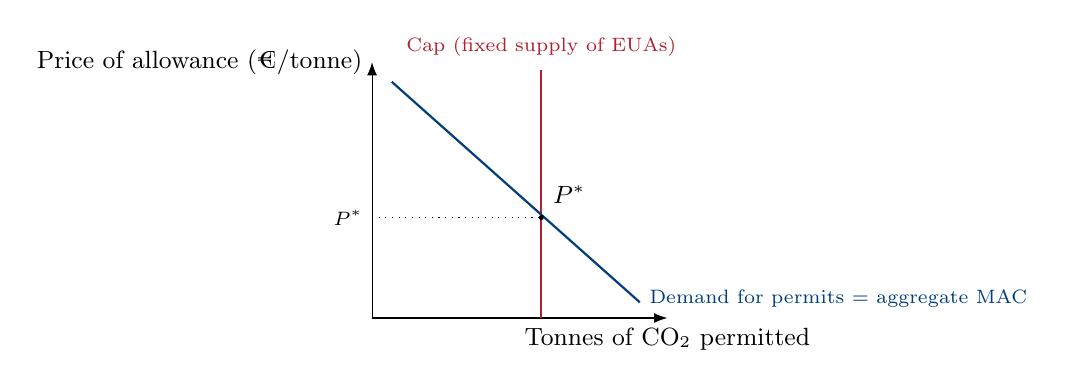
\begin{tikzpicture}[scale=0.5]
    \draw[-{Latex}] (0,0) -- (7.5,0) node[below, font=\small]{Tonnes of CO\textsubscript{2} permitted};
    \draw[-{Latex}] (0,0) -- (0,6.5) node[left, font=\small]{Price of allowance (\texteuro/tonne)};
    \draw[wured, thick] (4.3,0) -- (4.3,6.3);
    \node[above, font=\scriptsize, wured] at (4.3,6.4) {Cap (fixed supply of EUAs)};
    \draw[wublue, thick] (0.5,6) -- (6.8,0.4);
    \node[right, font=\scriptsize, wublue] at (6.8,0.5) {Demand for permits $=$ aggregate MAC};
    \fill (4.3,2.55) circle (1.8pt);
    \node[above right, font=\small] at (4.35,2.65) {$P^*$};
    \draw[dotted] (0,2.55) -- (4.3,2.55);
    \node[left, font=\scriptsize] at (0,2.55) {$P^*$};
  \end{tikzpicture}
  \end{center}
  \footnotesize The cap fixes the \emph{quantity} of permits (vertical supply). The downward-sloping ``demand for permits'' curve is really the aggregate \textbf{marginal abatement cost (MAC)} curve. The market finds $P^*$ on its own --- nobody has to know the MAC curve in advance, unlike with a Pigouvian tax.
\end{frame}

\begin{frame}{The Four Phases}
  \small
  \begin{center}
  \begin{tabular}{@{}p{1.6cm}p{2.0cm}p{9.0cm}@{}}
    \toprule
    \textbf{Phase} & \textbf{Years} & \textbf{Key feature} \\
    \midrule
    I & 2005--2007 & ``Learn by doing'' pilot; almost all allowances given away free, based on firms' own reported historical emissions. \\
    II & 2008--2012 & Aligned with the EU's Kyoto Protocol commitment; still mostly free allocation. \\
    III & 2013--2020 & First EU-wide cap (previously set by 27 separate national plans); auctioning becomes the default for the power sector. \\
    IV & 2021--2030 & Cap tightened sharply in line with the European Green Deal; Market Stability Reserve fully active; aviation and maritime scope expanded. \\
    \bottomrule
  \end{tabular}
  \end{center}
\end{frame}

% =============================================================
\section{Growing Pains: Getting the Design Right}

\begin{frame}{Phase I: Over-Allocation and the 2006--2007 Price Crash}
  \begin{itemize}
    \item Regulators set each country's cap based on firms' \textbf{self-reported} historical emissions --- and firms had every incentive to overstate them, to be handed generous free allowances.
    \item When verified 2005 emissions data came out in April 2006, it turned out the cap had been set \textbf{above} actual emissions --- there was no real scarcity.
    \item The permit price, which had traded around \texteuro{}30/tonne, collapsed toward \textbf{\texteuro{}0} by the end of Phase I.
  \end{itemize}
  \begin{alertblock}{The lesson}
    A cap-and-trade system is only as good as the cap. Get the quantity wrong --- through bad information or political pressure to be generous --- and you get the price of an unregulated good: zero.
  \end{alertblock}
\end{frame}

\begin{frame}{Phase II--III: The 2008 Crisis and a Decade of Oversupply}
  \begin{itemize}
    \item The 2008 financial crisis sharply reduced industrial output --- and with it, emissions --- well below the Phase II cap.
    \item Allowance prices fell from $\approx$\texteuro{}25 to the single digits, and a large \textbf{surplus} of unused permits accumulated and carried over into Phase III.
    \item Result: for most of the 2010s, EUA prices stayed low (roughly \texteuro{}5--8/tonne) --- too low to meaningfully drive abatement investment.
  \end{itemize}
  \small This is the classic \textbf{price-volatility problem} with a pure quantity instrument: an external demand shock (a recession) that has nothing to do with the environment still swings the permit price violently, because the \emph{quantity} of permits was fixed without foreseeing the shock.
\end{frame}

\begin{frame}{The Fix: The Market Stability Reserve (2019)}
  \begin{block}{Market Stability Reserve (MSR)}
    An automatic mechanism that withholds allowances from auctions when the total surplus in circulation is too high, and releases them back when the surplus is too low.
  \end{block}
  \begin{itemize}
    \item Directly targets the oversupply left over from the 2008 crash.
    \item Effectively blends a pure quantity instrument with a bit of \emph{price-stabilizing} flexibility --- the system's own answer to the price-vs-quantity trade-off from the theory lecture.
    \item Alongside a much steeper post-2021 cap reduction (the ``Fit for 55'' package), the MSR helped push EUA prices from single digits up past \texteuro{}50 by 2021, briefly touching nearly \texteuro{}100/tonne in early 2023.
  \end{itemize}
\end{frame}

\begin{frame}{Free Allocation vs.\ Auctioning}
  Recall the first key difference between taxes and tradable permits: \textbf{how the permits are initially allocated}.
  \begin{itemize}
    \item \textbf{Free allocation (``grandfathering'')}, as in Phases I--II: equivalent to a Pigouvian tax \emph{plus} a large transfer to incumbent polluters --- the environmental incentive is the same, but existing firms are handed a windfall.
    \item \textbf{Auctioning}, the Phase III--IV default for power generation: equivalent to a pure Pigouvian tax --- the government captures the revenue instead of handing it to polluters.
  \end{itemize}
  \small The EU ETS has moved steadily from (i) toward (ii) over 20 years --- a real-world illustration of exactly the allocation choice covered in theory, and of how politically difficult auctioning is to introduce all at once.
\end{frame}

\begin{frame}{Carbon Leakage: Why Some Free Allocation Remains}
  \begin{block}{Carbon leakage}
    If EU firms face a carbon price but foreign competitors don't, production --- and the emissions that come with it --- may simply relocate outside the EU, with \emph{no} net environmental benefit.
  \end{block}
  \begin{itemize}
    \item Energy-intensive, trade-exposed sectors (steel, cement, chemicals) still receive a substantial share of allowances \textbf{free}, specifically to blunt this relocation incentive.
    \item This is a real cost of \emph{unilateral} climate policy --- exactly the international-coordination problem from the climate-change section of the externalities lecture: one region acting alone bears a competitiveness cost that a coordinated global carbon price would not.
  \end{itemize}
\end{frame}

% =============================================================
\section{Does It Actually Work?}

\begin{frame}{Empirical Evidence: Did the EU ETS Cut Emissions?}
  \begin{itemize}
    \item \textbf{Ellerman \& Buchner} and related early studies estimate emissions from covered installations were roughly \textbf{8--12\% lower} cumulatively over Phase I--II than a no-ETS counterfactual --- a modest but real effect, achieved despite the well-documented Phase I price collapse.
    \item \textbf{Bayer \& Aklin (2020)}, using a synthetic-control design, estimate the EU ETS avoided roughly \textbf{1 billion tonnes of CO\textsubscript{2}} between 2008--2016 relative to a no-policy counterfactual --- even through the years of very low permit prices.
  \end{itemize}
  \small Takeaway: even an imperfectly designed, low-priced permit market did \emph{some} of what theory predicts --- but a much higher, more stable price (as in Phase IV) should do substantially more.\\
  \srcnote{Ellerman \& Buchner (2008), \emph{Review of Environmental Economics and Policy}; Bayer \& Aklin (2020), \emph{PNAS} 117(16).}
\end{frame}

\begin{frame}{Empirical Evidence: Effects on Innovation and Competitiveness}
  \textbf{Calel \& Dechezleprêtre (2016)} compare EU ETS--regulated firms to similar unregulated firms.
  \begin{itemize}
    \item Regulated firms increased \textbf{low-carbon patenting} by roughly \textbf{10\%} more than comparable unregulated firms --- consistent with the corrective-tax logic that a real carbon price induces genuine technological response, not just short-run output cuts.
    \item No detectable negative effect on regulated firms' overall economic performance (employment, revenue) relative to unregulated firms --- an important reply to the ``carbon pricing kills industry'' worry.
  \end{itemize}
  \srcnote{Calel \& Dechezleprêtre (2016), \emph{Review of Economics and Statistics} 98(1).}
\end{frame}

% =============================================================
\section{What's Next: The Carbon Border Adjustment Mechanism}

\begin{frame}{CBAM: Attacking Carbon Leakage Directly}
  \begin{block}{Carbon Border Adjustment Mechanism (CBAM)}
    A tariff-like charge on imports of specific carbon-intensive goods (steel, cement, aluminum, fertilizers, electricity, hydrogen), set equal to the carbon price EU producers already pay --- phasing in fully by 2026.
  \end{block}
  \begin{itemize}
    \item Directly targets carbon leakage --- the ``stick'' side of the rich-country decarbonization toolkit from the climate-change lecture --- as an \textbf{alternative} to free allocation, rather than living alongside it forever.
    \item As CBAM phases in, free allocation for the sectors it covers is meant to phase \emph{out} --- moving the EU ETS closer to a ``pure'' auctioned permit system even for exposed industries.
  \end{itemize}
\end{frame}

% =============================================================
\begin{frame}{Discussion Questions}
  \begin{enumerate}
    \setlength{\itemsep}{8pt}
    \item Phase I gave away permits based on self-reported emissions, which firms had an incentive to inflate. What alternative allocation rule would have been harder to game --- and what would it have cost politically?
    \item The 2008 price crash happened because a demand shock (recession) hit a fixed-quantity instrument. Would a \emph{carbon tax} have handled the 2008 shock better or worse than the EU ETS did? Under what conditions?
    \item Is CBAM a better long-run solution to carbon leakage than free allocation --- or does it just shift the problem to trade disputes with non-EU countries?
  \end{enumerate}
\end{frame}

% =============================================================
\begin{frame}{Sources}
  \tiny
  \begin{columns}[T]
    \begin{column}{0.5\textwidth}
      Bayer, P. \& Aklin, M. (2020), \emph{PNAS} 117(16).\\
      Calel, R. \& Dechezleprêtre, A. (2016), \emph{Review of Economics and Statistics} 98(1).\\
      Ellerman, A.D. \& Buchner, B. (2008), \emph{Review of Environmental Economics and Policy} 2(1).
    \end{column}
    \begin{column}{0.5\textwidth}
      European Commission, ``EU Emissions Trading System (EU ETS)'' (policy overview, ec.europa.eu).\\
      Gruber, J., \emph{Public Finance and Public Policy}, Ch.\ 5.\\
      Saez, E., \emph{Econ 131} lecture notes, UC Berkeley.
    \end{column}
  \end{columns}
\end{frame}

\begin{frame}[standout]
  Thank you!\\
  \vspace{0.5em}
  \small Questions and discussion
\end{frame}

\end{document}
